% Uncomment this to make slides with overlays:
%\documentclass[slides]{beamer}

% Uncomment these (but comment the above \documentclass line) to make handouts:
\documentclass[handout]{beamer}

% Uncomment these to have more than one slide per page
%\usepackage{pgfpages}
%\pgfpagesuselayout{2 on 1}[border shrink=5mm]
%\pgfpageslogicalpageoptions{1}{border code=\pgfusepath{stroke}}
%\pgfpageslogicalpageoptions{2}{border code=\pgfusepath{stroke}}

\usepackage[]{graphicx, color, hyperref}

\mode<presentation>
{
	%\usetheme[secheader]{Boadilla}
	%\usecolortheme[rgb={.835, .102,.169}]{structure}  
	\usetheme[width= 0cm]{Goettingen}
	%\setbeamercovered{transparent}
}
\setbeamertemplate{navigation symbols}{}
\setbeamertemplate{footline}[frame number]

\definecolor{blue2}{rgb}{0.278,0.278,0.729} 
\newcommand{\blue}[1]{\textcolor{blue2}{#1}}
\newcommand{\white}[1]{\textcolor{white}{#1}}
\newcommand{\red}[1]{\textcolor{red}{#1}}
\newcommand{\xbar}{\overline{x}}
\newcommand{\ybar}{\overline{y}}
\newcommand{\phat}{\widehat{p}}
\newcommand{\prob}{\mbox{Pr}}
\newcommand{\E}{\mathbb{E}}
\newcommand{\Var}{\mbox{Var}}
\newcommand{\cp}{\oplus}
\newcommand{\cm}{\circleddash}


\title{Lecture 20: ANOVA Part II}
\author{Chapter 5.5}
\date{}


\begin{document}
%------------------------------------------------------------------------------
\begin{frame}
\titlepage
\end{frame}
%------------------------------------------------------------------------------


%-------------------------------------------------------------------------------
\begin{frame}
\frametitle{Previously: Conditions for Using t Distribution}
%
% Comment this
%
We use the $t$ distribution when you have

\begin{itemize}
\pause \item $n$ is small. E.g. 3, 5, 10, 15.
\pause \item \blue{Independence}: $n \leq 10\% $ rule
%or if we have an experiment or random process we check that each observation were independent
\pause \item \blue{Observations come from a nearly normal distribution}:
\begin{itemize}
\item Look at a histogram of the data (difficult when $n$ is small)
\item Consider whether any previous experiences alert us that the data may be normal
\end{itemize}
\end{itemize}  
	
\end{frame}
%-------------------------------------------------------------------------------


%------------------------------------------------------------------------------
\begin{frame}[fragile]
\frametitle{New Topic: Analysis of Variance (ANOVA)}
A farmer has the choice of four tomato fertilizers and wants to compare their performance in terms of crop yield.

\pause \vspace{0.5cm}

We have $k=4$ groups AKA \blue{levels of a factor}: the 4 types of fertilizer.  \pause Say we:
\begin{itemize}
\pause \item assign $n_i$ plants to each of the $k=4$ fertilizers as follows:
\[
\begin{array}{cccc|c}
n_1 & n_2 & n_3 & n_4 &\mbox{total }n\\
\hline
3 & 7 & 4 & 6 & 20
\end{array}
\]
\pause \item we evaluate the number of tomatoes on each plant
\end{itemize}

\end{frame}
%------------------------------------------------------------------------------


%-------------------------------------------------------------------------------
\begin{frame}
\frametitle{Tomato Fertilizer}
We observe the following, where each point is one tomato plant. \textcolor{white}{Plot the sample mean of each level.} \textcolor{white}{Question: are the mean tomato yields different?}  
\setkeys{Gin}{width=0.65\textwidth}
\begin{center}
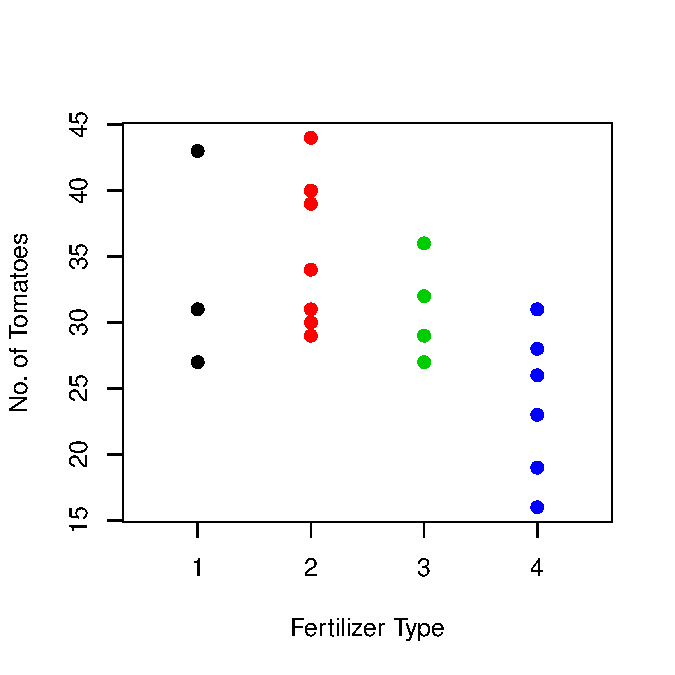
\includegraphics{figure/lec22-003}
\end{center}
\end{frame}
%-------------------------------------------------------------------------------


%-------------------------------------------------------------------------------
\addtocounter{framenumber}{-1}
\begin{frame}
\frametitle{Tomato Fertilizer}
We observe the following, where each point is one tomato plant.  Plot the sample mean of each level. \textcolor{white}{Question:  are the mean tomato yields different?} 
\setkeys{Gin}{width=0.65\textwidth}
\begin{center}
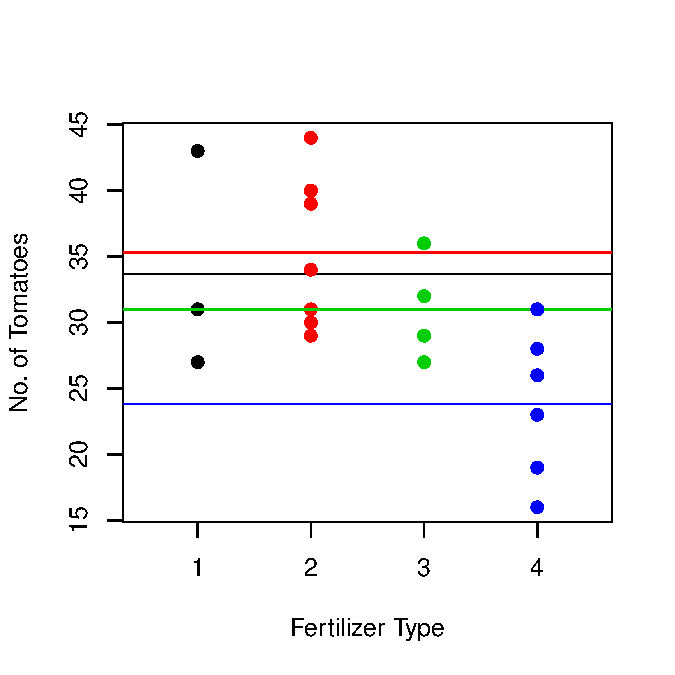
\includegraphics{figure/lec22-004}
\end{center}
\end{frame}
%-------------------------------------------------------------------------------


%-------------------------------------------------------------------------------
\addtocounter{framenumber}{-1}
\begin{frame}
\frametitle{Tomato Fertilizer}
We observe the following, where each point is one tomato plant.  Plot the sample mean of each level. \blue{Question:  are the mean tomato yields different?}
\setkeys{Gin}{width=0.65\textwidth}
\begin{center}
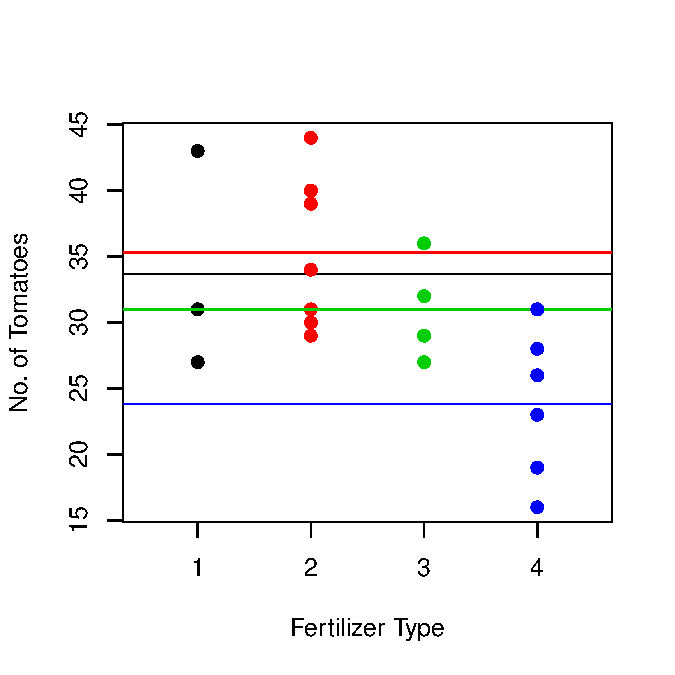
\includegraphics{figure/lec22-004}
\end{center}
\end{frame}
%-------------------------------------------------------------------------------


%-------------------------------------------------------------------------------
\begin{frame}
\frametitle{Analysis of Variance}
Say we have $k$ groups and want to compare the $k$ means:
\[
\mu_1, \mu_2, \ldots, \mu_k
\]

\pause \vspace{0.5cm}

We could do ${k \choose 2}$ individual two-sample tests.  \pause Ex. for groups 1 \& 2:
\begin{eqnarray*}
H_0: && \mu_1 = \mu_2\\
\mbox{vs. } H_a:  && \mu_1 \neq \mu_2
\end{eqnarray*}
\pause i.e. no difference in means

\end{frame}
%-------------------------------------------------------------------------------


%-------------------------------------------------------------------------------
\begin{frame}
\frametitle{Analysis of Variance}
Or, rather than conducting all ${k \choose 2}$ tests, we do \blue{a single overall test} via \blue{Analysis of Variance ANOVA}:

\vspace{0.5cm}

\pause The hypothesis test is:
\begin{eqnarray*}
H_0: && \mu_1 = \mu_2 = \ldots = \mu_k\\
\mbox{vs. } H_a:  && \mbox{at least one of the $\mu_i$'s are different}\\
\end{eqnarray*}
\end{frame}
%-------------------------------------------------------------------------------


%-------------------------------------------------------------------------------
\begin{frame}
\frametitle{How ANOVA Tests Work}
ANOVA asks:  where is the overall variability of the data originating from?

\vspace{0.5cm}

\pause The \blue{test statistic} used to compute a $p$-value is now the \blue{F-statistic}:
\[
F = \frac{\mbox{measure of between-group variability}}{\mbox{measure of within-group variability}}
\]
\end{frame}
%-------------------------------------------------------------------------------


%-------------------------------------------------------------------------------
\begin{frame}
\frametitle{Tomato Fertilizer Example}
Numerator: the \blue{between-group variation} refers to the variability \blue{between} the levels (the 4 horizontal lines):  
\setkeys{Gin}{width=0.65\textwidth}
\begin{center}
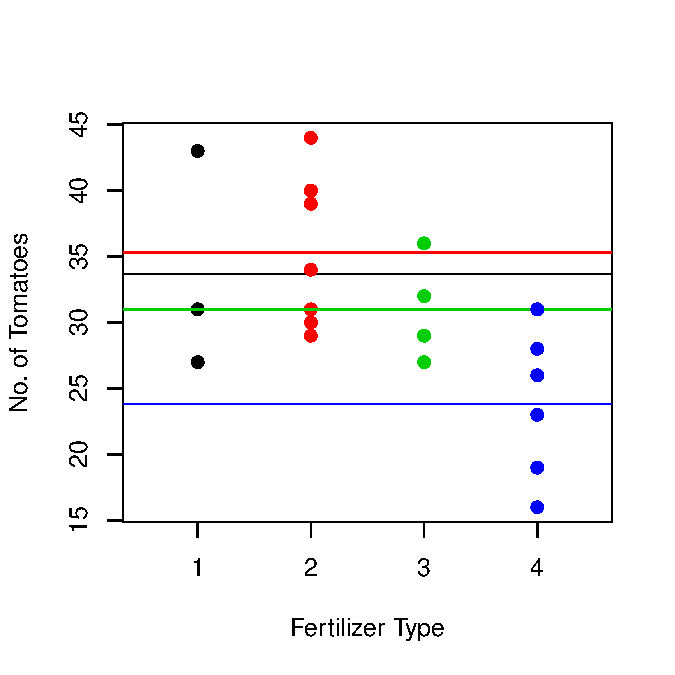
\includegraphics{figure/lec22-006}
\end{center}
\end{frame}
%-------------------------------------------------------------------------------


%-------------------------------------------------------------------------------
\begin{frame}
\frametitle{Tomato Fertilizer Example}
Denominator: the \blue{within-group variation} refers to the variability \blue{within} each level (the 4 vertical arrows):
\setkeys{Gin}{width=0.65\textwidth}
\begin{center}
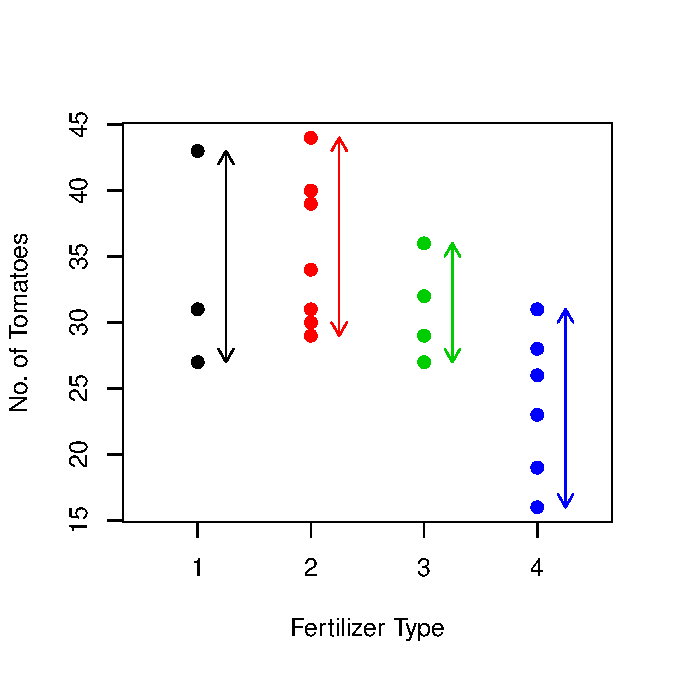
\includegraphics{figure/lec22-005}
\end{center}
\end{frame}
%-------------------------------------------------------------------------------


%-------------------------------------------------------------------------------
\begin{frame}
\frametitle{Tomato Fertilizer Example}
Now compare the following two plots:
\setkeys{Gin}{width=0.8\textwidth}
\begin{center}
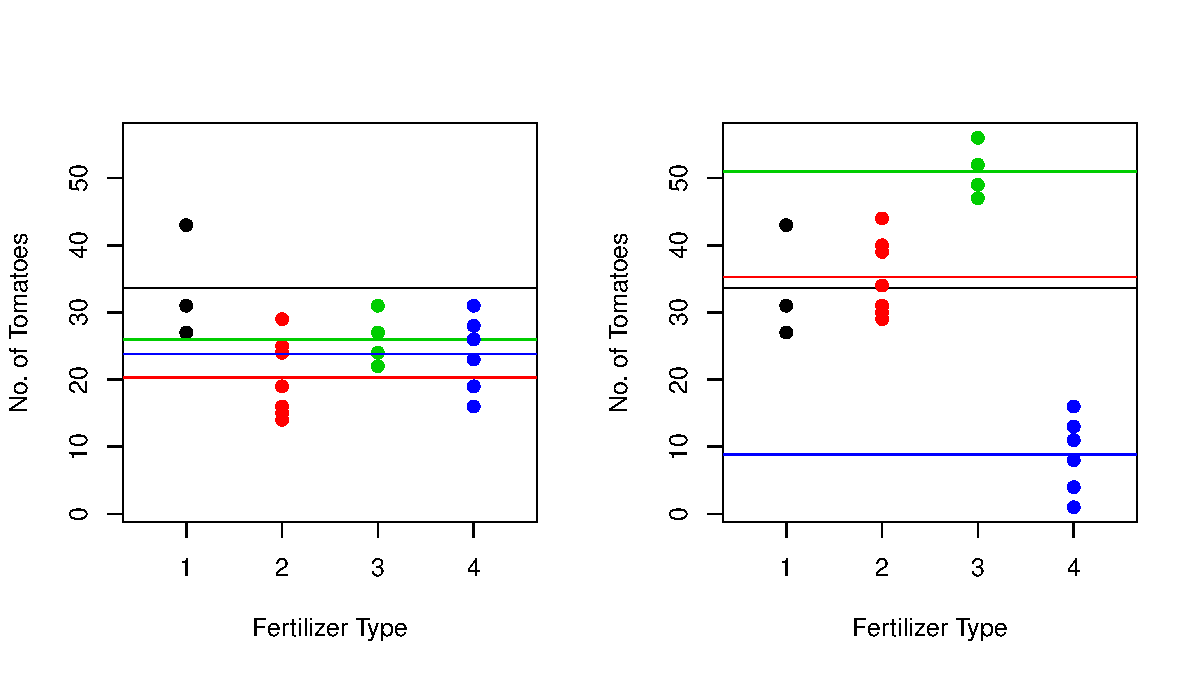
\includegraphics{figure/lec22-008}
\end{center}

\begin{itemize}
\pause \item They have the \blue{same within-group} variability.  Call this value $W$
\pause \item The right plot has \blue{higher between group variability}  b/c the 4 means are more different.  Call these values $B_{left}$ and $B_{right}$ with $B_{left} < B_{right}$
\end{itemize}

\end{frame}
%-------------------------------------------------------------------------------


%-------------------------------------------------------------------------------
\begin{frame}
\frametitle{Tomato Fertilizer Example}
\setkeys{Gin}{width=0.8\textwidth}
\begin{center}
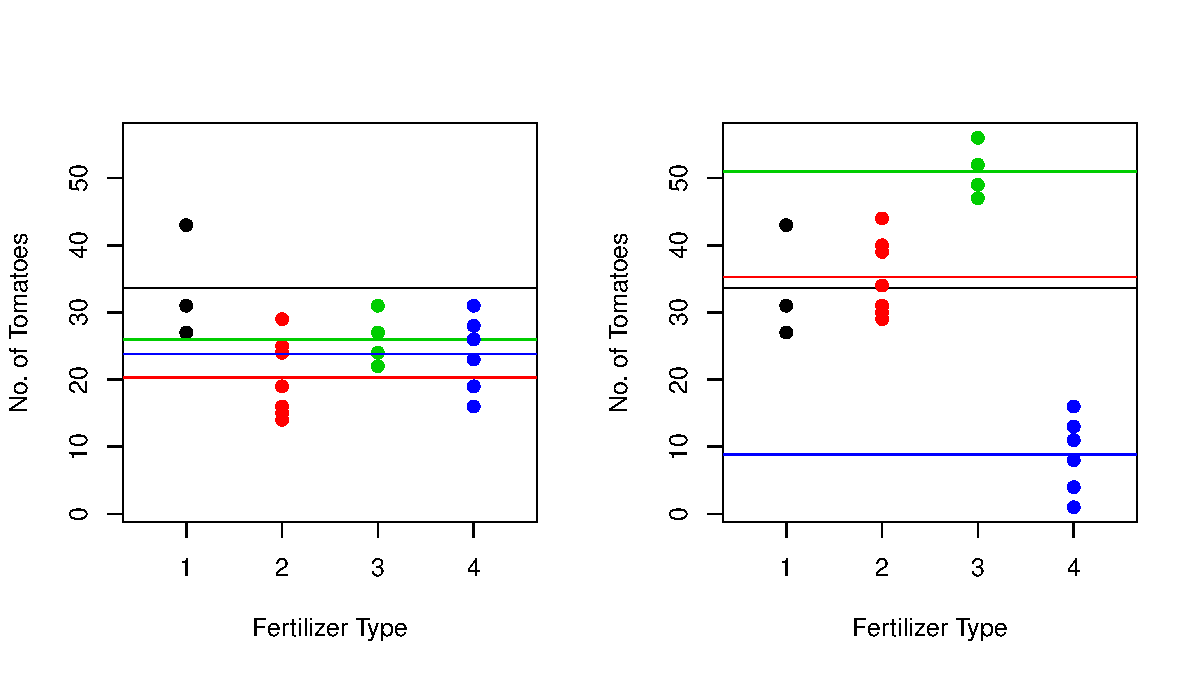
\includegraphics{figure/lec22-008}
\end{center}
\[
\pause \mbox{Recall }F = \frac{\mbox{measure of between-group variability}}{\mbox{measure of within-group variability}} 
\]
\pause \begin{eqnarray*}
\mbox{Since \ }\frac{B_{left}}{W} &<& \frac{B_{right}}{W}\\
\mbox{thus \ \ \  }F_{left} &<& F_{right}
\end{eqnarray*}

\end{frame}
%-------------------------------------------------------------------------------\


%-------------------------------------------------------------------------------
\begin{frame}
\frametitle{$F$ Distributions}
\blue{Assuming $H_0$ is true} (that $\mu_1 = \mu_2 = \ldots = \mu_k$), the $F$-statistic
\[
F = \frac{\mbox{measure of between-group variability}}{\mbox{measure of within-group variability}}
\]
follows the \blue{$F$ distribution with degrees of freedom $df_1=k-1$ and $df_2=n-k$} where
\begin{itemize}
\pause \item $n$ is the \blue{total} number of observations
\item $k$ is the number of groups
\end{itemize}
 
\end{frame}
%-------------------------------------------------------------------------------


%-------------------------------------------------------------------------------
\begin{frame}
\frametitle{$F$ Distributions}
Much like the $t$ distribution with degrees of freedom $df$, the parameters for the $F$ distribution are $df_1=k-1$ and $df_2=n-k$.  Example with $df_1 = 4$ and $df_2=6$:
\setkeys{Gin}{width=0.65\textwidth}
\begin{center}
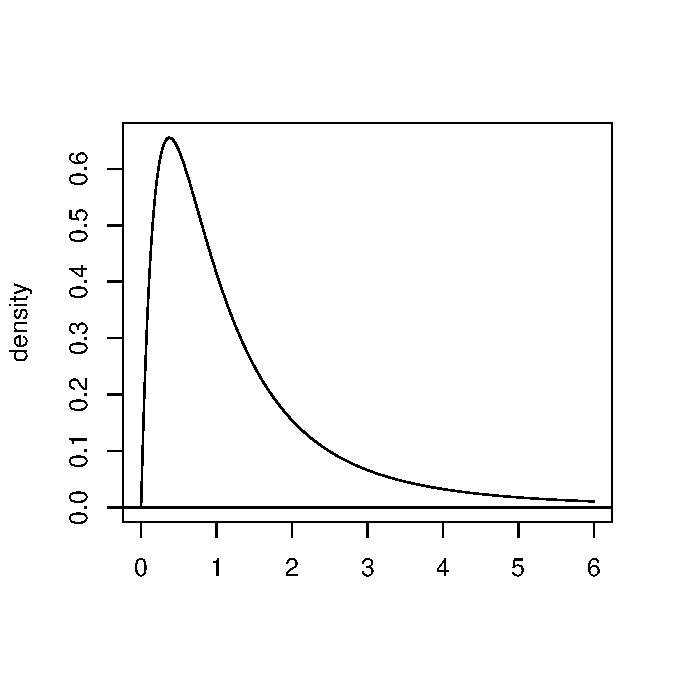
\includegraphics{figure/lec22-009}
\end{center}
\end{frame}
%-------------------------------------------------------------------------------


%-------------------------------------------------------------------------------
\begin{frame}
\frametitle{$F$ Distributions}
$p$-values are computed as before where ``more extreme'' means \blue{larger}.  You can compute these in {\tt R} using {\tt pf(F,df1,df2)}.  Say the $F$-statistic is equal to $3$, the $p$-value is the \blue{area to the right of 3}.
\setkeys{Gin}{width=0.65\textwidth}
\begin{center}
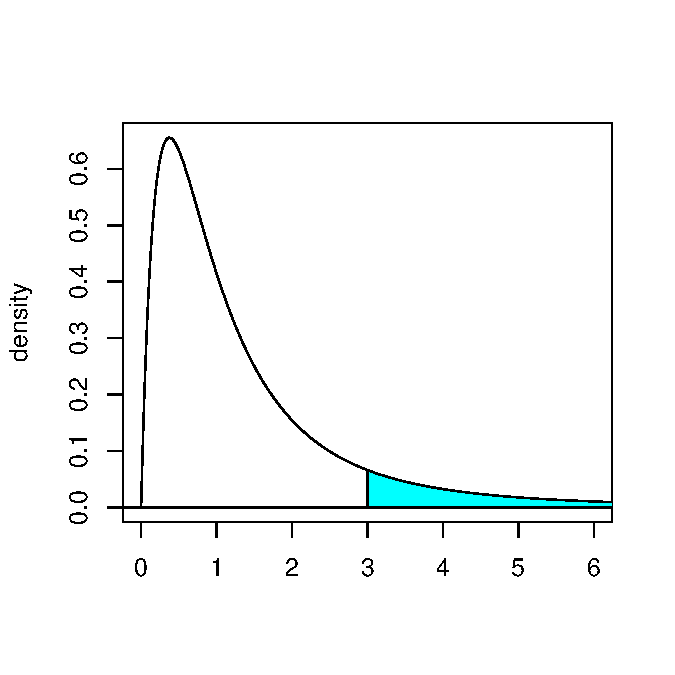
\includegraphics{figure/lec22-010}
\end{center}
\end{frame}
%-------------------------------------------------------------------------------


%-------------------------------------------------------------------------------
\begin{frame}
\frametitle{Conducting An $F$-Test}
The results are typically summarized in an \blue{ANOVA table}:

\begin{small}
\begin{center}
\begin{tabular}{l|ccc|cc}
Source of Variation & $df$ & $SS$ & $MS$ & $F$ & $p$-value\\
\hline
Between groups & $k-1$ & $SSTr$ & $MSTr = \frac{SSTr}{k-1}$ & $\frac{MSTr}{MSE}$ & $p$\\
Within groups & $n-k$ & $SSE$ & $MSE = \frac{SSE}{n-k}$ & & \\
\hline
Total & $n-1$ & $SST$ &  & & 
\end{tabular}
\end{center}
\end{small}
\end{frame}
%-------------------------------------------------------------------------------


%-------------------------------------------------------------------------------
\begin{frame}
\frametitle{Conditions}
\begin{enumerate}
\pause \item The observations have to be \blue{independent}.  10\% rule.  
\pause \item If the sample sizes are small within each group, \blue{normality} of the data is important.  If not small, we can be lax about this. 
\pause \item Each of the groups has \blue{constant variance} $\sigma_1^2 = \ldots = \sigma_k^2 = \sigma^2$.  We can check this with boxplots and by comparing the sample standard deviations $s_1, \ldots, s_k$
\end{enumerate}

\end{frame}
%-------------------------------------------------------------------------------


%------------------------------------------------------------------------------
\begin{frame}[fragile]
\frametitle{Discussion of Yesterday's Quiz}
Question 1:  Why did 1 out of the 20 studies yield a positive/significant result i.e. that there is a link between jelly beans and acne?

\vspace{0.25cm}


\pause Not that the p-value is 0.05, rather that \blue{$\alpha=0.05$} (significance level AKA type I error rate AKA false positive rate) \\
\pause i.e. we expect 1 out of 20 results to be significant 


\end{frame}
%------------------------------------------------------------------------------


%------------------------------------------------------------------------------
\begin{frame}[fragile]
\frametitle{Publication Bias}
\blue{Publication bias}: people only highlight significant/positive results.  \pause From Wikipedia: ``Publication bias occurs when the publication of research results \blue{depends on their nature and direction}.''

\vspace{0.5cm}

\pause To counter this, some prominent medical journals (incl. the New England Journal of Medicine, The Lancet, Annals of Internal Medicine, and JAMA) require registration of a trial \blue{before} it starts so that unfavorable results are not withheld from publication. 

\vspace{0.5cm}

\pause \blue{\url{http://www.jnrbm.com/content/10/1/6}}

\end{frame}
%------------------------------------------------------------------------------


%------------------------------------------------------------------------------
\begin{frame}[fragile]
\frametitle{Publication Bias}

\begin{center}
\pause 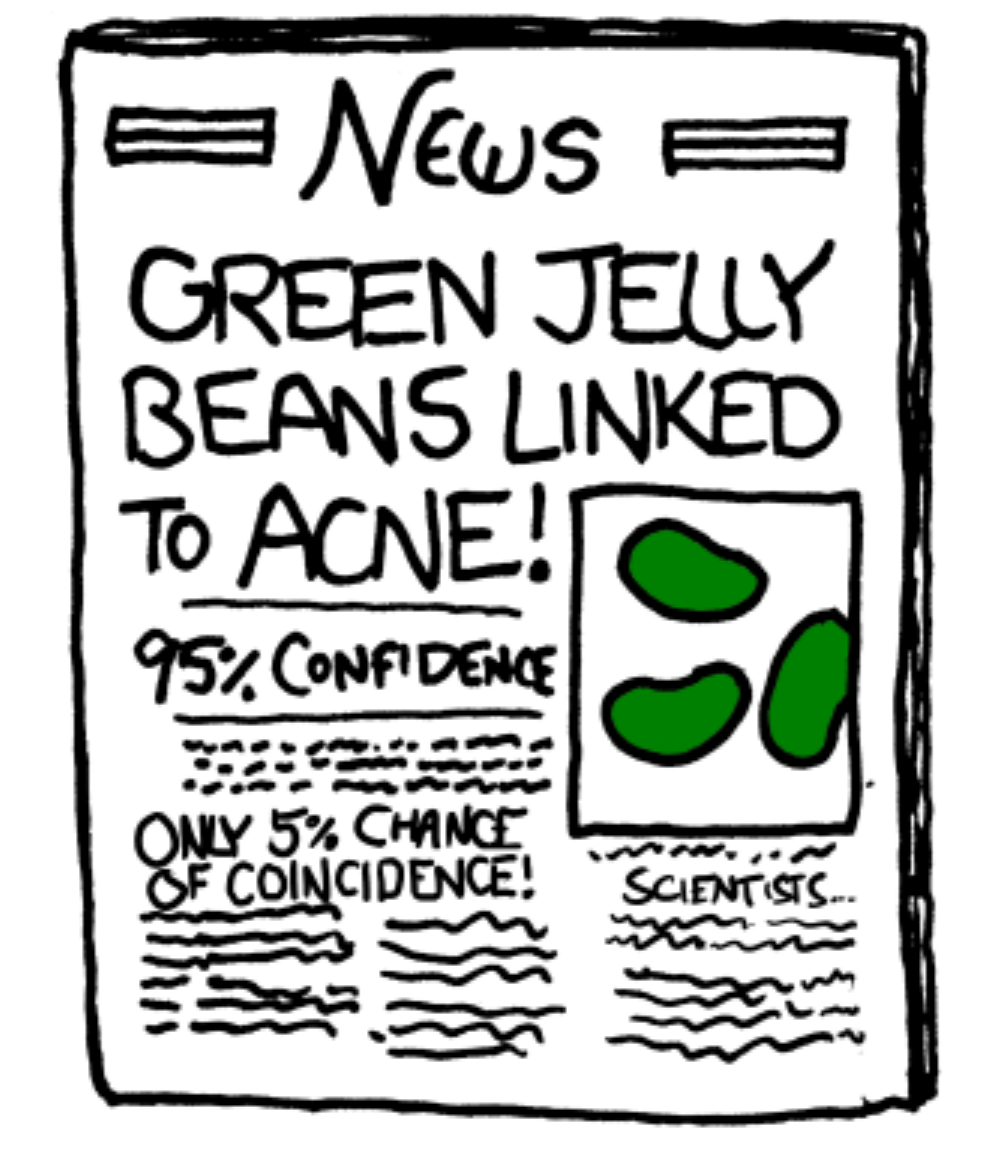
\includegraphics[width=0.5\textwidth]{figure/jelly.png}
\end{center}

\end{frame}
%------------------------------------------------------------------------------


%------------------------------------------------------------------------------
\begin{frame}[fragile]
\frametitle{Publication Bias}

\begin{center}
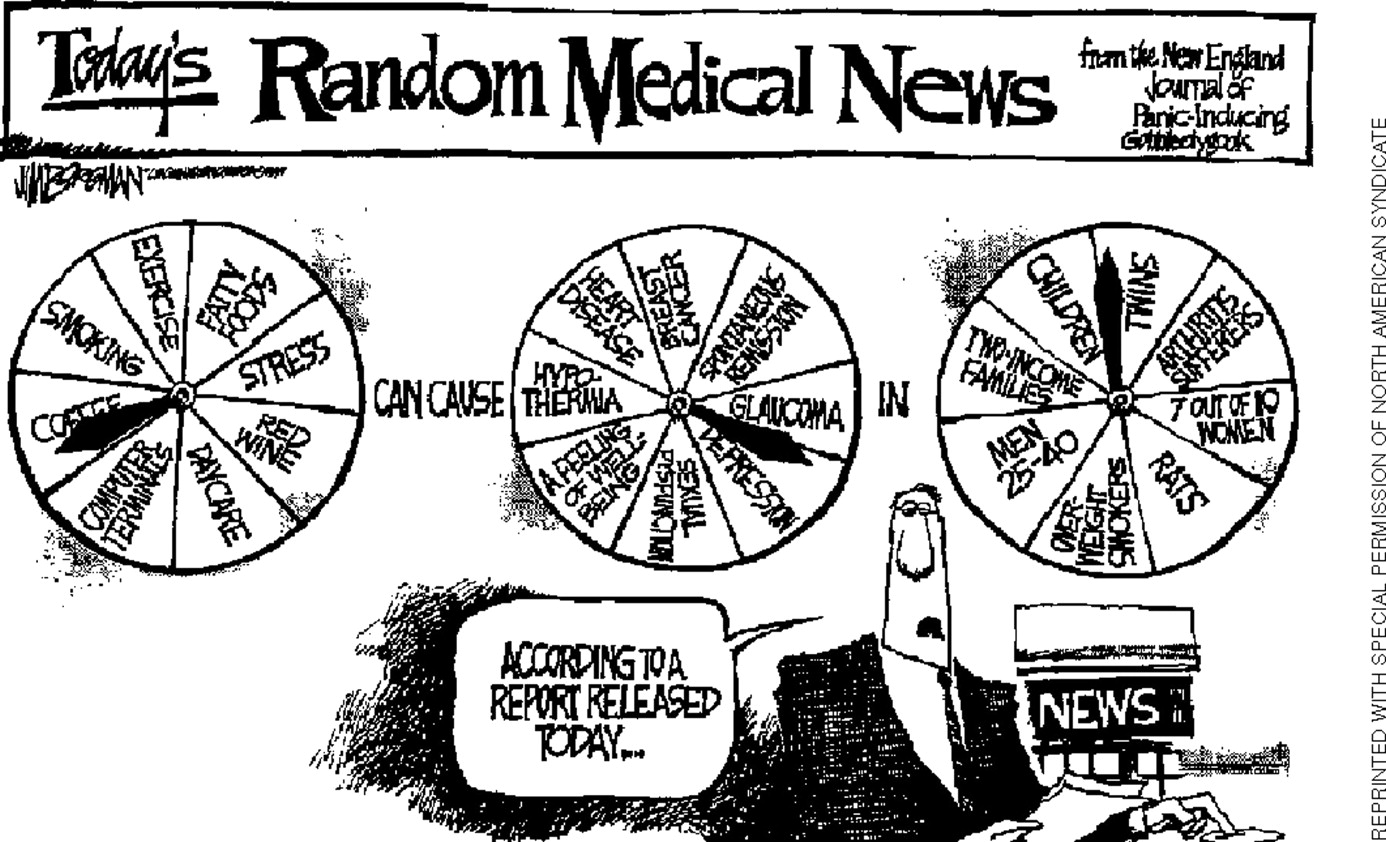
\includegraphics[width=\textwidth]{figure/wheel.jpg}
\end{center}
From:  Sterne JA, Davey Smith G (2001) Sifting the evidence - What's wrong with significance tests. BMJ 322: 226�231.
\end{frame}
%------------------------------------------------------------------------------


%------------------------------------------------------------------------------
\begin{frame}[fragile]
\frametitle{Multiple Testing}
A related issue is the statistical concept of \blue{multiple testing}.

\vspace{0.5cm}

\pause Say the null is true (i.e. nothing is going on).  If you repeat the experiment more and more times, you're bound to get a significant result eventually just by \blue{chance alone}.

\end{frame}
%------------------------------------------------------------------------------


%------------------------------------------------------------------------------
\begin{frame}[fragile]
\frametitle{Multiple Testing}
You conduct $n=20$ tests of different jelly beans colors at the $\alpha=0.05$ significance level.  We expect 5\% of them to be significant by chance alone.  

\pause \vspace{0.5cm}

If the tests are independent, the number of significant tests is \blue{Binomial}$(n=20, p=\alpha=0.05)$.  

\pause \vspace{0.5cm}

We saw in Chapter 3 
\[\mu = np = 20 \times 0.05 = 1 \mbox{ test}\]

\end{frame}
%------------------------------------------------------------------------------


%------------------------------------------------------------------------------
\begin{frame}[fragile]
\frametitle{Multiple Testing}
What is
\begin{eqnarray*}
P(\mbox{at least one sig result in 20}) &=& \pause 1 - P(\mbox{no sig results in 20})\\
\pause &=& 1 - {20 \choose 0} \alpha^{0} (1-\alpha)^{20} \\
\pause &=& 1- (1-0.05)^{20}\\
\pause &\approx& 0.64
\end{eqnarray*}

\pause We have 64\% chance of observing at least one significant result, even if ``nothing is going on.''

\vspace{0.25cm}

\pause Why?  Because we did so many tests!  That is a huge chance of a false positive!
\end{frame}
%------------------------------------------------------------------------------


%------------------------------------------------------------------------------
\begin{frame}[fragile]
\frametitle{Multiple Testing}

What do people do?  Make the $\alpha$ stricter!  i.e. 
\begin{itemize}
\pause \item make the $\alpha$ smaller
\pause \item so we have less chance the p-value is smaller than $\alpha$
\pause \item so we have less chance of incorrectly rejecting the null when it is true
\end{itemize}

\vspace{0.25cm}

\pause \blue{Bonferroni correction}:  If you are conducting $n$ tests, use $\alpha^* = \frac{\alpha}{n}$

\end{frame}
%------------------------------------------------------------------------------


%------------------------------------------------------------------------------
\begin{frame}[fragile]
\frametitle{Multiple Testing}
So in our case, use $\alpha^* = \frac{0.05}{20} = 0.0025$.  \pause Now
\begin{eqnarray*}
P(\mbox{at least one sig result in 20}) &=& \pause 1 - P(\mbox{no sig results in 20})\\
&=& 1 - {20 \choose 0} \alpha^{*0} (1-\alpha^{*})^{20} \\
&=& 1- (1-0.0025)^{20}\\
&\approx& 0.0488
\end{eqnarray*}

\pause Closer to \blue{true desired} $\alpha=0.05$.  

\vspace{0.25cm}

\pause \blue{Note}: the correction is conservative in that the overall type I error rate is $0.0488 < 0.05$.

\end{frame}
%------------------------------------------------------------------------------


%------------------------------------------------------------------------------
\begin{frame}[fragile]
\frametitle{What $\alpha$ To Set for Single Tests}
About using $\alpha=0.05$ as your significance level.  Before using it, at least put \blue{some} thought into the balance between:
\begin{itemize}
\pause \item \blue{Type I errors}.  If type I errors matter more, set $\alpha$ small.
\pause \item \blue{Type II errors}.  If type II errors matter more, set $\alpha$ high.
\end{itemize}

\end{frame}
%------------------------------------------------------------------------------



\end{document}










